\section{Tecnologías implementadas y estado operativo.}
\subsection{Análisis de RAM}
\label{subsec:ramanalisi}
Uno de los puntos más importantes a la hora de implementar un bot con IA para un juego de Atari, es entender cómo está hecho. Utilizaremos el entorno \ac{ale} para extraer características de los juegos, el cual cuenta con una API que nos permite extraer información de los mismos. Para ello, se ha desarrollado un lector de RAM que nos ayuda a visualizar los 128 bytes de memoria de la Atari mientras se ejecuta un juego.

Además, dicho lector implementa colores, lo cual permite que se puedan distinguir las posiciones de RAM que cambian de las que no en un step determinado (paso de ejecución)  como se puede ver en la figura \ref{fig:RAM_Colors}.

\begin{figure}[h]
	\centering
	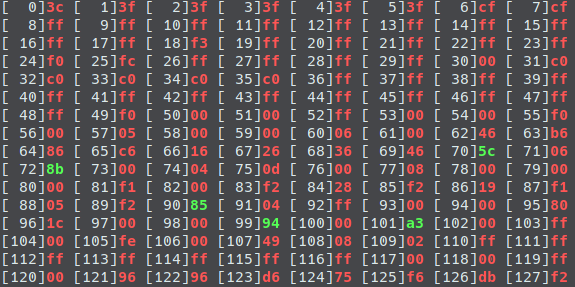
\includegraphics[width=1\textwidth]{Figures/RAMColors}
	\caption{El color verde indica que el valor ha cambiado en este step.}
	\label{fig:RAM_Colors}
\end{figure}

Una de las características de este lector es que acompaña la ejecución con un volcado de analytics para ver las posiciones de RAM que más han cambiado en una ejecución determinada.

Para extraer los datos mas interesantes de un juego en concreto, simplemente hay que observar las posiciones de RAM mas alteradas según nuestro analytics. Una vez hecho esto, se pondrá el juego en cámara lenta gracias a una feature del entorno \ac{ale}, lo cual nos permitirá ver con qué sentido cambian estos valores. Como punto a destacar, no todos los valores que cambian mucho serán relevantes a la hora de sacar datos importantes del juego (un contador podría no ser relevante para un caso específico).

Una vez hecho esto se puede desglosar la RAM de manera bastante precisa, sacando datos como los siguientes.

\begin{figure}[h]
	\centering
	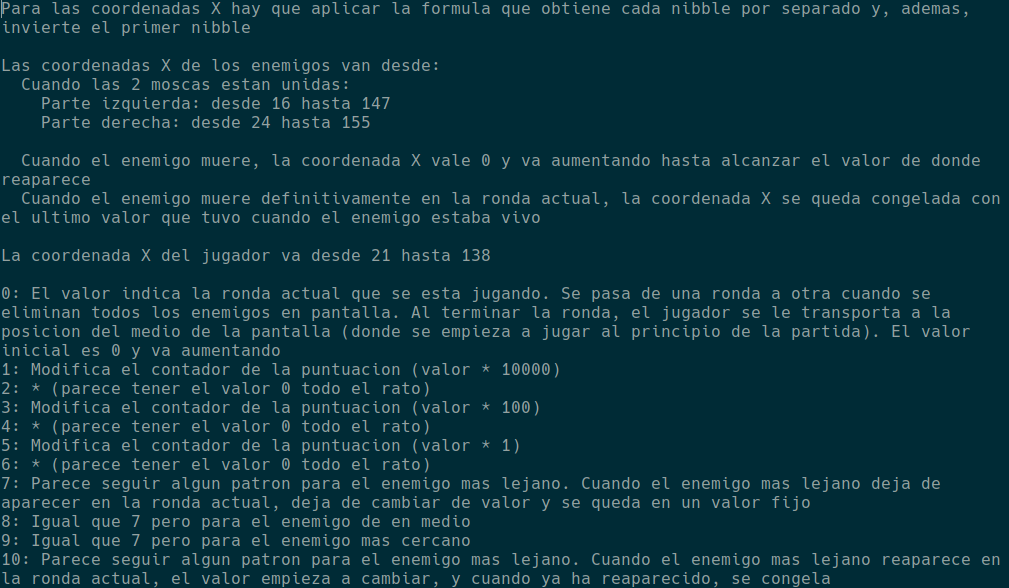
\includegraphics[width=1\textwidth]{Figures/AnalisisRAM}
	\caption{Demon Attack - Análisis de las primeras posiciones de RAM}
	\label{fig:AnalisisRAM}
\end{figure}

Como se puede observar en la figura \ref{fig:AnalisisRAM}, para obtener la información correcta no solo basta con extraer las posiciones relevantes, en algunos casos será necesario procesar esta información. Por ejemplo, en Demon Attack, las coordenadas X de las entidades aparecen obfuscadas de la siguiente manera:

\begin{figure}[h]
	\centering
	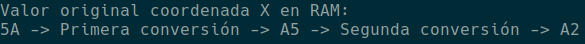
\includegraphics[width=1\textwidth]{Figures/DAttackOpsRequired}
	\caption{Demon Attack - Coordenadas X de las entidades}
	\label{fig:DAttackOpsRequired}
\end{figure}

Como podemos ver en la figura \ref{fig:DAttackOpsRequired}, los nibbles de las coordenadas están invertidos, además, el primer nibble requiere una operacion extra, una resta (7 - valor del nibble). 

Una vez tenemos la información recogida y procesada, la podremos utilizar para crear una IA capaz de jugar al juego en concreto. Además de eso, el entorno \ac{ale} cuenta con diversas funcionalidades que nos permiten recoger la información en pantalla en el caso que fuese necesario. 

\subsubsection{Modificando ALE}
\label{subsubsec:ramanalisi:modale}
Lorem ipsum dolor sit amet, consectetur adipiscing elit. Curabitur diam quam, placerat sit amet ornare ut, dignissim non orci. Suspendisse et pellentesque sem, id facilisis magna. Morbi consequat blandit ipsum, sed accumsan ex vehicula quis. Maecenas interdum malesuada neque, non laoreet magna dignissim a. Vivamus rhoncus enim eget neque pretium, condimentum hendrerit leo venenatis. Vestibulum elementum semper sem a ultricies. Pellentesque habitant morbi tristique senectus et netus et malesuada fames ac turpis egestas. Nullam pulvinar pellentesque quam viverra consectetur. Donec sit amet enim eu ante porttitor commodo elementum eget orci. Duis lobortis mattis nibh, sodales feugiat sapien efficitur sed. Duis ultrices turpis eu nisl maximus, id luctus justo elementum. Curabitur porttitor nec nibh at ullamcorper.

Aliquam egestas elit vitae faucibus tincidunt. Donec dolor nulla, congue quis lobortis quis, euismod at elit. Phasellus viverra auctor augue nec luctus. Aenean elementum facilisis sapien, a imperdiet lacus maximus varius. Mauris in maximus urna. Mauris quis varius mi, id commodo nibh. Vivamus et quam ultrices, sollicitudin justo a, egestas mauris.

Aenean ut egestas ipsum. Praesent placerat ex sit amet mauris eleifend auctor sit amet tincidunt nibh. Fusce in varius justo, eget euismod tortor. Pellentesque sagittis bibendum mi, vel mollis dolor congue a. Nulla vitae pharetra ex, quis commodo justo. Cras a volutpat nisi, vitae lobortis sem. Aenean ullamcorper, erat eget vehicula tempor, magna nunc rhoncus turpis, ac commodo dolor risus id sem. Morbi efficitur vel felis at finibus. Nullam tristique erat id est ornare, sed finibus libero bibendum. Cras at tellus ligula. Ut eget pretium ante, condimentum tristique nisi.

Quisque condimentum nunc id nisi sollicitudin elementum et at diam. Etiam facilisis cursus urna, mollis euismod magna efficitur at. Praesent ullamcorper varius accumsan. Sed quis est id orci sollicitudin sollicitudin. Donec consectetur, ante quis eleifend ultrices, risus turpis efficitur justo, eget fermentum ipsum nisi ac ipsum. Integer accumsan facilisis viverra. Aliquam id nisl faucibus, pharetra dui vel, venenatis elit. Morbi auctor, magna ac pellentesque fringilla, urna ex aliquam velit, ut lacinia enim diam nec augue. Nulla posuere auctor imperdiet. Praesent cursus cursus erat, ac varius odio vulputate in. Morbi ultricies consequat ex, eu convallis purus pretium non. Duis tincidunt nibh eget fermentum auctor.

\newpage
\subsection{Bots básicos}
\label{subsec:botsbasicos}
Se han desarrollado bots semi-deterministas empleando técnicas básicas de inteligencia artificial para poder extraer datos de gameplay. Los primeros volcados de datos se hicieron con operarios humanos jugando a los juegos, pero al ver que nuestras scores eran mas bien bajas, se optó por implementar IA básica para cada uno de los juegos. 

Estas implementaciones básicas mejoraron mucho las scores obtenidas, por lo que los datos extraidos de los bots eran mas afines a obtener mayores puntuaciones que los nuestros.

Además, sobre esta IA básica, se pueden hacer iteraciones de mejora, teniendo en cuenta más datos o mas información en pantalla, como se ha comentado anteriormente en la subsección \ref{subsec:ramanalisi}.

Este scripting básico ayudará mas adelante a la implementación utilizando machine learning, ya que los datos extraidos y procesados para la implementación básica serán utilizados por el algoritmo de machine learning.

A continuación, describiremos cada uno de los bots básicos y su funcionamiento al igual que algunos detalles de implementación.

\subsubsection{Plantilla común}
\label{subsec:botsbasicos:plantcomun}
Todos los bots comparten una serie de utils que analizaremos a continuación.

\begin{figure}[h]
	\centering
	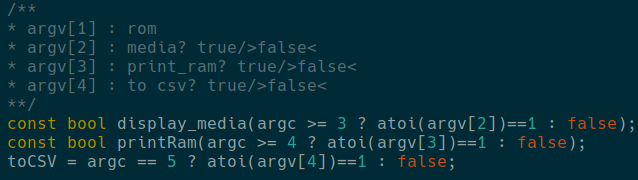
\includegraphics[width=1\textwidth]{Figures/ALEMediaSettings}
	\caption{Opciones de ejecución}
	\label{fig:ALEMediaSettings}
\end{figure}

argv 1 es la rom que utilizará nuestro ejecutable, argv 2 se corresponde con el contenido multimedia (video y audio), argv 3 escribirá la RAM en consola y argv 4 exportará los datos de gameplay a un archivo \ac{csv} si así se requiere. Se han parametrizado estas opciones porque las ejecuciones son mucho mas lentas conforme mas información requiramos, esto se nota sobre todo a la hora de desactivar el contenido multimedia.

\begin{figure}[h]
	\centering
	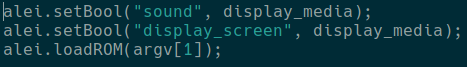
\includegraphics[width=0.7\textwidth]{Figures/ALEromANDmedia}
	\caption{La ROM y el contenido multimedia corren a cargo de \ac{ale}.}
	\label{fig:ALEromANDmedia}
\end{figure}

\newpage
Algunas de estas opciones corren a cargo del entorno (Figura 	\ref{fig:ALEromANDmedia}), mientras que las otras han sido implementadas por nosotros.

Otra de las partes comunes a todos los bots es el bucle principal de ejecución que podemos ver a continuación en la figura \ref{fig:ALEMainExecLoop}. Este bucle está situado en \textbf{main()} y es el encargado de analizar y ejecutar las acciones requeridas en cada step del juego en activo.

\begin{figure}[h]
	\centering
	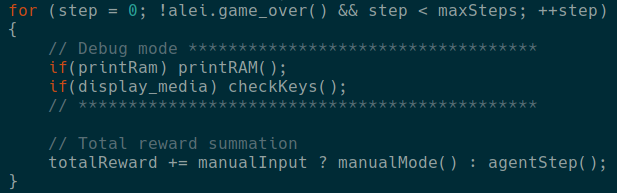
\includegraphics[width=1\textwidth]{Figures/ALEMainExecLoop}
	\caption{Bucle principal de ejecución.}
	\label{fig:ALEMainExecLoop}
\end{figure}

En este bucle observamos nuestra opción \textbf{printRam} que llama al método encargado de imprimir la RAM, el cual convierte a hexadecimal cada uno de los valores de RAM obtenidos mediante el método \textbf{getRAM().get(i)} del entorno \ac{ale}, además hace un seguimiento de los valores de ram del step anterior para comprobar si dichos valores han cambiado como hemos visto anteriormente en la figura \ref{fig:RAM_Colors}.

Otra opción que encontramos en el bucle principal de ejecución es \textbf{display\_media}, pero en este caso es usado para llamar al método \textbf{checkKeys()}, esto se hace porque no tiene sentido trackear el input si no existe contenido de video. Este método de input es propio, ya que el método de input de ALE "pausa" el agente, lo cual no nos interesa para extraer datos. \textbf{checkKeys()} simplemente activa o desactiva el modo manual propio con la tecla "E", reflejado en la variable \textbf{manualInput}.

La variable \textbf{manualInput} decidirá que función se llama para calcular \textbf{totalReward}. \textbf{manualMode()} mapea el teclado a diferentes acciones del juego, mientras que \textbf{agentStep()} es el bot autónomo específico a cada juego.

Otra de las partes comunes a todos los agentes es la parte de volcado de datos, para ello se han implementado dos funciones de escritura que imprimen strings o dobles en el archivo \ac{csv} anteriormente comentado, como bien podemos ver en la figura .

\begin{figure}[h]
	\centering
	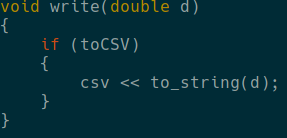
\includegraphics[width=0.4\textwidth]{Figures/aledumpcsv}
	\caption{Una de las funciones de escritura en CSV.}
	\label{fig:aledumpcsv}
\end{figure}


\subsubsection{Breakout}
\label{subsec:botsbasicos:breakout}
El Breakout es el juego mas simple de todos los que analizaremos en esta parte de la sección, pues el número de inputs que tiene es mas bien pequeño. En el Breakout contamos con un total de 5 vidas para pasarnos los 2 niveles de los que dispone. El Breakout fue el primer juego en el que vimos la necesidad de automatizar al jugador, ya que la velocidad de la pelota va incrementando en funcion a los ladrillos restantes que quedan, lo cual provocaba que perdiesemos siempre en este punto.

\begin{figure}[h]
	\centering
	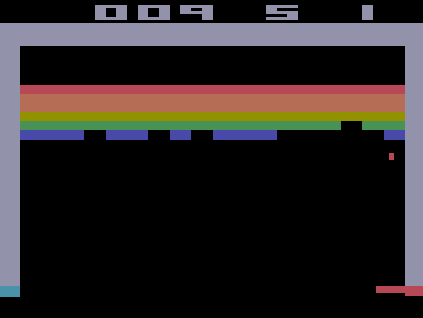
\includegraphics[width=0.7\textwidth]{Figures/breakoutgame}
	\caption{Juego Breakout.}
	\label{fig:breakoutgame}
\end{figure}

Simplemente proporcionando la posición X de la pelota y de la pala al bot naive y moviendo la pala hacia la pelota, el agente ya jugaba bastante bien. Una mejora que se hizo al algoritmo es hacer un control del tamaño de la pala, al igual que en vez de tener en cuenta solo la posicion actual de la pelota, añadir a los datos la posición anterior. Con todas estas mejoras la puntuación se maximizó hasta el punto en el cual el agente fue capaz de pasarse el juego completo. A continuacion se muestra en el algoritmo \ref{alg:breakoutimpl}
el pseudocódigo de la IA del Breakout.

\vspace{4mm}
\begin{algorithm}[H]
	\If{lives() != lastLives}{
		$--$lastLives\;
		act(FIRE)\;
	}
	
	wide := getRAM.get(108)\;
	playerX := getPlayerX()\;
	ballX := getBallX()\;
	
	\If{$BallX\_LastTick < ballX$}{
		ballX $+= ((rand() \% 2) + 2);$
	}
	\If{$BallX\_LastTick > ballX$}{
		ballX $-= ((rand() \% 2) + 2);$
	}

	ballX\_LastTick := getBallX()\;
	
	\eIf{$ballX < playerX + wide$}{
		reward $+= act(LEFT);$
	}{
		\If{$(ballX > playerX + wide) \&\& (playerX + wide < 188)$}{
			reward $+= act(RIGHT);$
		}
	}
	\caption{Breakout agent}
	\label{alg:breakoutimpl}
\end{algorithm}

Si analizamos el pseudocódigo anterior, podemos ver cuatro partes. En la primera parte, constituida por el primer if, vemos como el agente presiona la tecla \textbf{FIRE} cuando pierde una vida, esto se debe a que en Breakout cuando pierdes una vida tienes que sacar la pelota pulsando esa tecla. 

En la segunda parte recogemos los datos principales, en este caso \textbf{wide}, que corresponde al ancho de la pala, además de \textbf{playerX} y \textbf{ballX}. 

La tercera parte calcula la dirección de la bola, esto se saca comprobando la posicion anterior de la bola con la actual en el eje X, una vez sabemos la direccion aplicamos una suma con un poco de aleatoriedad (para evitar ejecuciones deterministas) en la dirección recogida. Una vez hecho eso nos guardamos la posicion de la pelota para la siguiente iteración.

En la cuerta parte aplicaremos el input en funcion a la posicion del jugador respecto a la pelota, teniendo en cuenta el ancho de la pala recogido anteriormente.

\subsubsection{Boxing}
\label{subsec:botsbasicos:boxing}
Boxing es un juego en el cual controlamos a un boxeador y tenemos que asestar mas golpes que el rival para ganar la ronda. En este juego tuvimos los mismos problemas que con el Breakout, por lo que decidimos implementar otro bot, el cual jugaba mejor que nosotros, lo que se resumia en todo ventajas.

\begin{figure}[h]
	\centering
	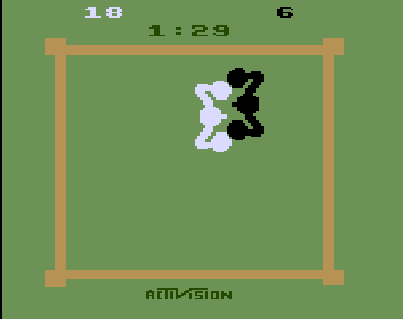
\includegraphics[width=0.7\textwidth]{Figures/boxing}
	\caption{Juego Boxing.}
	\label{fig:boxing}
\end{figure}

En este agente hemos tomado una estrategia agresiva, si el rival lanza un puñetazo, lo intentaremos bloquear con nuestros propios puños poniendo a nuestro boxeador exactamente en la misma posición "Y" que el boxeador contrario (una de las features de Boxing es que la colisión de los puños bloquea los golpes). Además, nuestro boxeador nunca se moverá hacia la izquierda, solo se mueve hacia la derecha en posición de ataque intentando posicionarse en la "Y" del rival, como hemos comentado antes. A su vez, basandonos en ciertas tolerancias, se atacará siempre que sea posible. Esta estrategia agresiva funciona una gran mayoria de las veces, además para evitar el determinismo se ha implementado una pequeña aleatoriedad cada vez que recogemos las posiciones del jugador 1 y del jugador 2 de RAM, como bien se puede ver en el ejemplo de la figura \ref{fig:boxingAleatoriedad}.

\begin{figure}[h]
	\centering
	\includegraphics[width=0.7\textwidth]{Figures/boxingAleatoriedad}
	\caption{Uso de \textbf{rand()} para evitar el determinismo.}
	\label{fig:boxingAleatoriedad}
\end{figure}

A continuación se muestra en el algoritmo \ref{alg:boxingimpl}, la IA implementada. Un detalle a comentar antes de entrar a analizar el algoritmo es que \textbf{player\_pos} es un tipo de dato struct.

%\vspace{2mm}
\begin{algorithm}[H]
	player\_pos p1(getP1\_X(), getP1\_Y())\;
	player\_pos p2(getP2\_X(), getP2\_Y())\;
	absp1p2X := abs(p1.x - p2.x)\;
	absp1p2Y := abs(p1.y - p2.y)\;
	
	\eIf{$absp1p2Y > 3$ \&\& $absp1p2Y < 20$}{
		reward $+= act(FIRE);$
	}{
		\eIf{$absp1p2X > 25$ \&\& $absp1p2X < 40$}{
			reward $+= act(RIGHT);$
		}{
			reward += $(p1.y > p2.y)$ ? act(UP) : act(DOWN)\;
		}
	}
	\caption{Boxing agent}
	\label{alg:boxingimpl}
\end{algorithm}

En la primera parte de recogida de datos, encapsulamos en un struct la posicion del jugador uno y la del jugador dos extrayéndolos de RAM, como ya hemos comentado anteriormente, estas posiciones implementan una aleatoriedad mínima para evitar ejecuciones deterministas. Además, en la misma sección, calcularemos la distancia entre ambos jugadores en "X" y en "Y", representadas en \textbf{absp1p2X} y \textbf{absp1p2Y} respectivamente, para luego utilizarlas mas adelante.

Una vez tenemos todos los datos procesados, observaremos si nos encontramos en un rango de tolerancia "Y" válido para atacar, si lo estamos, atacaremos (como punto a destacar, este rango es bastante amplio para enfatizar esta estrategia ofensiva). Si no podemos atacar, nos moveremos hacia la derecha  con ciertas tolerancias, o nos situamos en la "Y" del enemigo.


\subsubsection{Demon Attack}
\label{subsec:botsbasicos:da}
Lorem ipsum dolor sit amet, consectetur adipiscing elit. Curabitur diam quam, placerat sit amet ornare ut, dignissim non orci. Suspendisse et pellentesque sem, id facilisis magna. Morbi consequat blandit ipsum, sed accumsan ex vehicula quis. Maecenas interdum malesuada neque, non laoreet magna dignissim a. Vivamus rhoncus enim eget neque pretium, condimentum hendrerit leo venenatis. Vestibulum elementum semper sem a ultricies. Pellentesque habitant morbi tristique senectus et netus et malesuada fames ac turpis egestas. Nullam pulvinar pellentesque quam viverra consectetur. Donec sit amet enim eu ante porttitor commodo elementum eget orci. Duis lobortis mattis nibh, sodales feugiat sapien efficitur sed. Duis ultrices turpis eu nisl maximus, id luctus justo elementum. Curabitur porttitor nec nibh at ullamcorper.

Aliquam egestas elit vitae faucibus tincidunt. Donec dolor nulla, congue quis lobortis quis, euismod at elit. Phasellus viverra auctor augue nec luctus. Aenean elementum facilisis sapien, a imperdiet lacus maximus varius. Mauris in maximus urna. Mauris quis varius mi, id commodo nibh. Vivamus et quam ultrices, sollicitudin justo a, egestas mauris.

Aenean ut egestas ipsum. Praesent placerat ex sit amet mauris eleifend auctor sit amet tincidunt nibh. Fusce in varius justo, eget euismod tortor. Pellentesque sagittis bibendum mi, vel mollis dolor congue a. Nulla vitae pharetra ex, quis commodo justo. Cras a volutpat nisi, vitae lobortis sem. Aenean ullamcorper, erat eget vehicula tempor, magna nunc rhoncus turpis, ac commodo dolor risus id sem. Morbi efficitur vel felis at finibus. Nullam tristique erat id est ornare, sed finibus libero bibendum. Cras at tellus ligula. Ut eget pretium ante, condimentum tristique nisi.

Quisque condimentum nunc id nisi sollicitudin elementum et at diam. Etiam facilisis cursus urna, mollis euismod magna efficitur at. Praesent ullamcorper varius accumsan. Sed quis est id orci sollicitudin sollicitudin. Donec consectetur, ante quis eleifend ultrices, risus turpis efficitur justo, eget fermentum ipsum nisi ac ipsum. Integer accumsan facilisis viverra. Aliquam id nisl faucibus, pharetra dui vel, venenatis elit. Morbi auctor, magna ac pellentesque fringilla, urna ex aliquam velit, ut lacinia enim diam nec augue. Nulla posuere auctor imperdiet. Praesent cursus cursus erat, ac varius odio vulputate in. Morbi ultricies consequat ex, eu convallis purus pretium non. Duis tincidunt nibh eget fermentum auctor.



%----------------------------------------------------------------------------------------------%
%----------------------------------------------------------------------------------------------%
%----------------------------------------------------------------------------------------------%
%----------------------------------------------------------------------------------------------%
\newpage
\subsection{Redes neuronales}
\label{subsec:nn}


\newpage